\documentclass{article} % Document class
\usepackage{amsmath, bm, amssymb,amsthm,enumitem}
\usepackage{tikz}
\usetikzlibrary{arrows}
\usepackage{babel}[english]
\usepackage{pgfplots}
\usepackage{titlesec}
\pgfplotsset{compat=1.18}
\title{My bs notes}
\author{Makus}
\date{\today}
\begin{document} % Begin document content
\maketitle

% \grouping{<something>} acts similar to a ToC entry for \chapter*{<something>}
%\pgfplotsset{ standard/.style={ axis line style = thick, trig format=rad, enlargelimits, axis x line=middle, axis y line=middle, enlarge x limits=0.15, enlarge y limits=0.15, every axis x label/.style={at{(current axis.right of origin)},anchor=north west}, every axis y label/.style={at={(current axis.above of origin)},anchor=south east} } }

\setcounter{secnumdepth}{4}
\theoremstyle{theorem}
\newtheorem{theorem}{Theorem}[paragraph]
\titleformat{\paragraph}
{\normalfont\normalsize\bfseries}{\theparagraph}{1em}{}
\titlespacing*{\paragraph}
{0pt}{3.25ex plus 1ex minus .2ex}{1.5ex plus .2ex}
\renewcommand{\qedsymbol}{$QED$}
\theoremstyle{definition}
\newtheorem{definition}{Definition}
\tableofcontents
\section{Introduction}
    \begin{center}
        just random ass notes, separted by sections.
    \end{center}
    \subsection{forenotes}
    For the entire part of Computer Science, Chapter 3, the variable naming standard will be as follows:
    \begin{center}
        i is input\\ o is output
    \end{center}
    unless stated otherwise.
    \\Another note is that the $QED$, meaning \textit{quod erat demonstratum} in Latin, means ''it is demonstrated'' and marks the end of proofs.
\section{math}
    \subsection{general}
        \subsubsection{bases}
        given  \begin{center}
            $n$ = base of number representation\\
            $x$ = number that is represented in base $n$,
        \end{center}
        Then $\dfrac{x}{n}$ shiftes everything in $x$ towards the left by one and $x\cdot n$ shiftes everything to the right.
        \subsubsection{logrithmic base 2}
        when taking $\log_2(1+x)$ where $0<x \leq1$, the output is approx. $x$.\\
        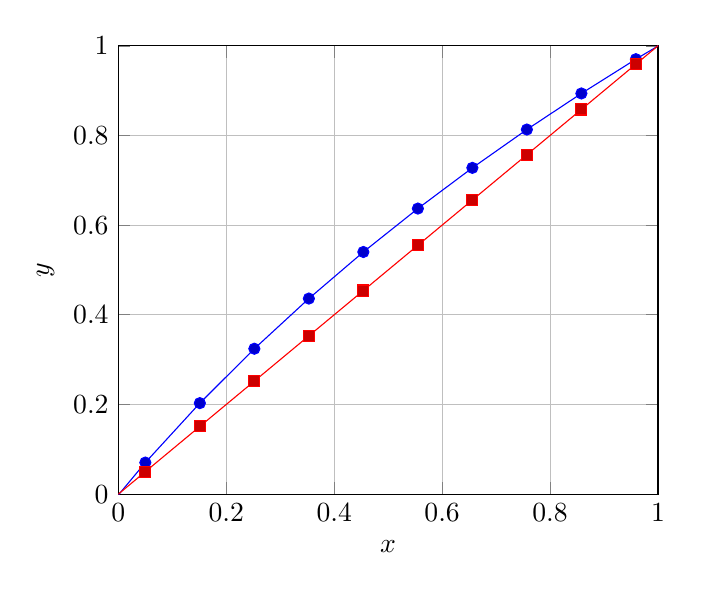
\begin{tikzpicture}
            \begin{axis}[
                xlabel={$x$},
                ylabel={$y$},
                samples=100,
                grid=major,
                xmin=0,xmax=1,
                ymin=0,ymax=1]
                \addplot{log10(x+1)/log10(2)};
                \addplot{x};
            \end{axis}
        \end{tikzpicture}
        \\but by adding $\mu$ to this, we can lower the amount of error to the average.
        to find $\mu$, we can do a mean value theorem stated in calculus portion to find $\mu$, which can be gotten from
        \begin{center}
            if$f(x)=\log_2(x+1)$, then $$f'(x)=\dfrac{1}{(x+1)\ln(2)}$$since the average rate of change is $$\dfrac{f(1)-f(0)}{1-0}=1$$
            then to get $\mu$, the steps are $$f'(c)=\dfrac{1}{(c+1)\ln(2)}=1$$ $$1=(c+1)\ln(2)$$ $$c=\dfrac{1}{\ln(2)}-1$$
            solving for c gives us the point on $f(x)$ where $f'(c)=1$
            \\given $c=\dfrac{1}{\ln(2)}-1$, then we can graph the tangent line with the point slope form.\\ $y-f(c)=f'(c)(x-c)$, or
            $$y=f(c)+f'(c)(x-c)$$ or $$y=f(c)-c+x$$ since $f'(c)=1$. since $f(c)-c$ is constant, it would be a straight line, modeled by the green line in the following
            the green line shows the tangent line with least error throughout. In order to find the overall average error, we can divide the sum of y intercepts by two in order to get the value of $\mu$, modeled by the blue line.
            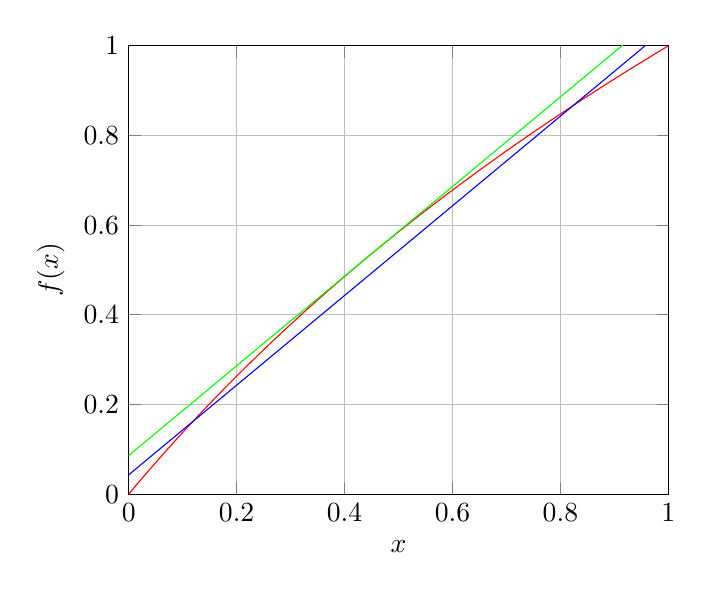
\begin{tikzpicture}
                \begin{axis}[xlabel={$x$},ylabel={$f(x)$},xmin=0, xmax=1,ymin=0,ymax=1,samples=1000,grid=major]
                    \addplot[color=red]{log10(x+1)/log10(2)};
                    \addplot[color=green]{x-(1/ln(2)-1)+log10(1/ln(2))/log10(2)} node[right]{$x+c$};
                    \addplot[color=blue]{x-((1/ln(2)-1)-log10(1/ln(2))/log10(2))/2};
                \end{axis}
            \end{tikzpicture}
            red is $\log_2(x+1)$\\
            green is $x+c-f(c)$, where $f(c)=\log_2(x+1)$\\
            blue is $x+\mu$, where $\mu=\dfrac{f(c)-c}{2}$
        \end{center}
    \subsection{calculus}
    this section will follow the order in which Calculus BC is taught, with first half from start of school to optimization problems, and second half being from integration to everything else.
        \subsubsection{First Half}
            \paragraph{Mean Value Theorem} % (fold)
            \label{ssub:Mean Value Theorem}
                    Mean Value Theorem, or MVT, states that if f(x) is continuous and differentiable within the range $a\le x \le b$, then there exists a point $c$ where $f'(c) = \dfrac{f(b)-f(a)}{b-a}$
        \subsubsection{Second Half}
            \paragraph{Unit 6}
                \subparagraph{Integration}
                    it is the inverse of differentiation, much like addition and subtraction. This process is denoted with the equation below.
                    $$\int f'(x)dx = f(x)$$
                    This shows the process of integration. A basic integration technique is Riemann sums.
                \subparagraph{Riemann Sums}
                    This is where we draw rectangles from the axis from which the function is in terms of up to a point of a function. Each subinterval's width can be given or can be calculated by a simple division. There are different types of Riemann sums.
                    It is not necessarily a rectangle, but it can also be a trapezoid, which is called the trapezoid Riemann Sum.
                    Some examples of Riemann Sums are:
                    \begin{itemize}
                        \item right corner: the height of the rectangle is equal to the value of the function at the right bound/limit, and can be modeled by the function $$\int_\alpha^\beta f(x)\approx \sum_{k=1}^{n}f(\alpha+k \cdot \Delta x)\cdot\Delta x$$
                        \item left corner: the height of the rectangle is equal to the value of the function at the left bound/limit, and can be modeled by the function $$\int_\alpha^\beta f(x) \approx \sum_{k=1}^{n}f(\alpha+(k-1)\cdot \Delta x)\cdot\Delta x$$
                        \item midpoint: the height of the rectangle is equal to the value of the function in the middle of the bound/limit, and can be modeled by the function $$\int_\alpha^\beta f(x)\approx \sum_{k=1}^{n}f(\alpha+(\Delta x\cdot(k-1))+(\frac{\Delta x}{2}))$$
                    \item trapezoid: instead of rectangles, trapezoids are used. This can be modeled by the function $$\int_\alpha^\beta f(x)\approx \sum_{k=1}^{n}(f(\alpha+(k-1)\cdot\Delta x)+f(\alpha+k\cdot\Delta x))\frac{\Delta x}{2}$$
                    \end{itemize}
                    where the variables are designed as
                    \begin{center}
                        $\Delta x$ is the width of the subinterval of each subinterval\\
                        $\alpha$ is the lower limit/bound of the integral\\
                        $\beta$ is the upper limit/bound of the integral\\
                        $n$ is the number of subintervals specified\\
                    \end{center}
                    Note: $n$ can be calculated if $\alpha$ and $\beta$
                    If something isn't integratable, then U-substitution can be used.
                \subparagraph{U substitution}
                    A variable can be used to replace a portion of a function. How this will work is:
                    \begin{enumerate}
                        \item Substitute a part of the function as u.
                        \item Where $u = f(x)$, the derivative would be $\dfrac{du}{dx} = f'(x)$, or $du = f'(x)dx$
                        \item Isolate dx an whatever way needed, then replace it back into the original function, so that the integral will be in terms of u (meaning it would be $\int du$)
                        \item After integrating, replace $u$ with $f(x)$
                    \end{enumerate}
                    Following these steps would look something like:
                    \begin{align*}
                        \int \dfrac{x}{\sqrt{1-4x^2}}dx \hspace{30px}
                        u &= 1-4x^2\\
                        \dfrac{du}{dx} &= 8x\\
                        du&=8xdx \\
                        \int \dfrac{1}{\sqrt{u}}du \hspace{80px}\\
                        \int u^{-1/2}du \hspace{70px}\\
                        \int u^{-\frac{1}{2}}du = \dfrac{u^{\frac{1}{2}}}{\frac{1}{2}}+c\hspace{30px}\\
                        2(1-4x^2)^{\frac{1}{2}}+c\hspace*{50px}
                    \end{align*}
                    If there are still $x$ values left after U-sub, then algabraic substitution can be used. This is where $u$ is expressed in terms of $x$.
                \subparagraph{Definite Integrals}
                    definite integrals output the area beneath the curve of the function, with the bounds of $\alpha$ and $\beta$, where $\alpha<\beta$. Notation denoted below:
                    $$\int_{\alpha}^{\beta}f'(x) dx = [f(x)]^{x=\alpha}_{x=\beta}$$ 
                    if $\alpha$ and $\beta$ are switched, then:
                    $$\int_{\beta}^{\alpha}f'(x) dx = -[f(x)]^{x=\alpha}_{x=\beta}$$
                    some more properties include:
                    \begin{enumerate}
                        \item $\int ^{\alpha}_{\alpha}f(x)dx = 0$
                        \item $\int _{\alpha}^{\beta}cf(x)dx =c\int _{\alpha}^{\beta}f(x)dx$(including negative numbers)
                        \item $\int _{\alpha}^{\beta}(f(x)\pm g(x))dx = \int _{\alpha}^{\beta}f(x)dx\pm \int _{\alpha}^{\beta} g(x)dx$
                        \item $\int _{\alpha}^{\beta}(f(x)dx)+\int ^{\gamma}_{\alpha}(f(x)dx)=\int ^{\gamma}_{\alpha}(f(x)dx)$
                        \item $\int ^{\alpha}_{-\alpha}f(x)dx=2\int ^{\alpha}_{0}f(x)dx$ assuming f(x) is even
                        \item $\int ^{\alpha}_{-\alpha}f(x)dx=0$ assuming f(x) is odd
                    \end{enumerate}
                \subparagraph{Fundamental Theorem of Calculus part 1}
                    If $f$ is continuous on $[a,b]$, then the following would be true:
                    \begin{equation}
                        \int^\beta_\alpha f'(x)dx = [f(x)]^{x=\beta}_{x=\alpha}=f(b)-f(a)
                    \end{equation}
                    Given this, it is possible to find either one of the three terms given two. 
                    \\\textbf{Keep In Mind}, when using U substitution and difinite integrals, the bounds need to change accordingly.
                    \begin{equation}
                        \int^\beta_\alpha f(u(x))u'(x)dx = \int^{u(\beta)}_{u(\alpha)}f(u)du
                    \end{equation}\pagebreak
            \paragraph{Unit 7}
                \subparagraph{Fundamental Theorem of Calculus Part 2}
                    \begin{theorem}[$FTC$ part 2]
                        \label{thm:FTCpt2}
                        assuming $f$ is continuous on $[\alpha,b]$, if $g(x)=\int_{\alpha}^{x}f(t)dt$, then $g'(x)=f(x)$, or \begin{equation} g'(x) = \frac{d}{dx}(\int_{\alpha}^{x}(f(t))dt) \end{equation}
                    \end{theorem}
                    \begin{proof}[Proof FTC Part 2]
                        This works the same way as $\int_{\alpha}^{\beta}f'(x)=f(x)$. \\Since $f(f^{-1}(x))=x$ and $f^{-1}(f(x))=x$, then this shows the proof \\of Theorem~\ref{thm:FTCpt2}.
                        Since derivatives and integrals are inverse functions of each other, this proves Theorem~\ref{thm:FTCpt2}.
                    \end{proof}
                    The Chain rule version of this theorem is \begin{equation}
                        \frac{d}{dx}\int_{a}^{g(x)}f(t)dt = f(g(x))g'(x)
                    \end{equation}
                \subparagraph{Logarithms}
                    Here are some rules regarding logs.
                    \begin{enumerate}
                        \item \textit{The domain of \emph{$\ln(x)$} is \emph{$(0,+\infty)$}.}
                        \item \textit{the range of \emph{$\ln x$} is $(-\infty,\infty)$}
                        \item $\lim_{x\rightarrow0^+}\ln(x)=-\infty$ and $\lim_{x\rightarrow+\infty}\ln(x)=+\infty$
                        \item \textit{the graph of \emph{$y=\ln x$} is continuous, increasing and one to one.}
                        \item \textit{the graph of \emph{$y=\ln x$} is concave downward.(\emph{$\frac{d^2}{dx^2}\ln x < 0$})}
                    \end{enumerate}
                    Here are some more theorems regarding $e$ and $\ln x$
                    \begin{enumerate}[label=(\alph*)]
                        \item \begin{equation} \lim_{x\rightarrow0}(1+x)^{\frac{1}{x}}=e \end{equation}
                        \item \begin{equation} \lim_{x\rightarrow +\infty}(1+\frac{1}{x})^x=e \end{equation}
                        \item \begin{equation} \lim_{x\rightarrow -\infty}(1+\frac{1}{x})^x=e \end{equation}
                    \end{enumerate}
                \subparagraph{Areas between Curve}
                    To find the area between the curves, the equation is \begin{equation}
                        A=\int_{\alpha}^{\beta}[f(x)-g(x)]dx
                        \label{eq:AreaBtCurve}
                    \end{equation}
                    where $x$ can be replaced with whatever variable, including $y$
                    
                    %\begin{definition}[Fundamental Theorem of Calculus Pt.2]
                     %   Suppose $f$ is coninuous on $[\alpha, \beta]$. if $g(x)=\int_{\alpha }^{max}$
                    %\end{definition}
        % subsubsection mean Value Theorem (end)
\section{Computer Science}\label{Computer Science}
will be using c++ for every example
    \subsection{bit shit}
        \subsubsection{bitwise operators to stop forgetting}
            \begin{center}
                \& is and\\$|$ is or\\$\wedge$ is xor\\$\sim$ for not\\$>>$ or $<<$ for moving bits left and right respectively
            \end{center}
            \paragraph{bitwise operator quirks?}
                In C++, every number is represented in binary, or base 2. Thus if anyone were to divide a number by two, then
                \begin{verbatim}
                    x=x>>1;//shifting towards the right
                \end{verbatim}
                works the same, but is faster. it also rounds up. Conversely, if anyone were to multiply by two, then 
                \begin{verbatim}
                    x=x<<1;//shifting towards the left
                \end{verbatim}
                does the same.
        \subsubsection{ieee 754}
            \paragraph{overview}
                This is how floats in C++ are stored. Floats are stored in 32 bit. the first bit is sign.
                The second to ninth bit is exponent, and the 10th to 32th bit is the mantissa. the exponent has
                an offset of 127, because it needs negative exponents. The mantissa, 23 bits, is the representation of the number(scientific notation).
                The equation to get from float to the final number is given by:
                \begin{equation}
                    (1+\dfrac{M}{2^{23}})\cdot2^{E-127}
                \end{equation}
            \paragraph{nitty griddy}
                The layout of this(the float) is 
                \begin{center}
                    sign bit:1 bit\\
                    exponent:1 byte(8 bits)\\
                    mantissa:23 bits\\
                \end{center}
                So if we were to follow this and try to extract exponents, we can do
                \begin{verbatim}
                    o = ((0xff<<23)&i)-127;
                \end{verbatim}
                and extracting the mantissa would be just 
                \begin{verbatim}
                    o = ((~(0xff<<23))&i);
                \end{verbatim}
                assuming the variables i and o are unsigned longs.
    \subsection{optimizations}
\section{physics}
    \subsection{Unit 4}
        \subsubsection{Work}
            \paragraph{definition}
                A force that causes an object to move. Units is $J$, $Joules$.
            \paragraph{rules}
                there are three rules for work to exist.
                \begin{itemize}
                    \item force must be applied
                    \item there must be a direction
                    \item there must be a displacement along the direction
                \end{itemize}
                \textbf{please Note:} 
                If the object that the force acts upon has no displacement, then said object has no work done onto it.
            \paragraph{equations}
                \begin{equation} W=fd \end{equation}
                \begin{equation} W=fd\cos(\theta) \end{equation}
                \begin{center} where $P$ is power \end{center}
                \begin{equation}
                    K=\frac{mv^2}{2}
                \end{equation}
        \subsubsection{power}
            \paragraph{definition}
                Power describes the rate of which work is performed.
                \begin{equation} P=\dfrac{\Delta w}{t} \end{equation}
        \subsubsection{Energy}
            \paragraph{Energy}
                the ability to do work.\\ Units is $J$, $Joules$.
                \subparagraph{Work Energy Theorem}
                    States that work can be converted to energy, $w=e$.
            \paragraph{Kinetic energy}
                Energy in motion. all moving objects have kinetic energy. $K$ represents kinetic energy.
                $$K=\frac{mv^2}{2}$$ 
            \paragraph{Gravitational potential energy}%
            \label{par:Gravitational potential energy}
                stored energy associated with an object's height above some reference point. $U_g$
                \begin{equation}
                    U_g=mgy
                \end{equation}
            \paragraph{Elastic potential energy}
                This describes the potential energy stored in the elastic material. $U_s$
                \begin{equation}
                    U_s=\frac{kx^2}{2}
                \end{equation}
                Where:\begin{center} $k$ is the spring constant\\$x$ is the distance from equilibrium \end{center}
            \paragraph{Mechanical Energy}
            It is the sum of potential and kinetic energy. It shows the sum of all energies present within an object.
        \subsubsection{Systems}
            A system is something some objects taken into consideration in a question where each object is described in relation to each other.
\end{document} % End document
